\chapter{Comments and Remarks} \label{ch:comments_and_remarks}

The following sections are intended to communicate any issues or remarks that arose throughout the acceptance testing process. They are concerned with the user interface, the documentation and code provided, and the implemented functionalities in general.

\section{Documentation Concerns}

\subsection{General Concerns}

\begin{itemize}
    \item Requirements and use cases look like they were not revised in further stages of the project, which leads to inconsistencies between them and the final product.
    \item Some use cases are missing. An example of such use case can be a farmer responding to a meeting request, which is mentioned in scenarios and use case diagrams, but not in use cases and requirements. This functionality is partially implemented, and always results in an error due to forbidden access, when trying to confirm/reject a meeting. This restricts possibility to test further functionalities, like meeting evaluation.
    \item Some of the terms are not explained clearly enough. An example of such a term can be \textit{Farm data}, which is only briefly mentioned in one paragraph of the DD.
    \item The Sign Up functionality, described in \textbf{U8} is available only for farmers. There is no possibility to add a new agronomist inside the \textit{Agronomist's WebApplication} is available only for farmers as stated in the provided documents. During testing, there was only one agronomist utilized, that was added using the provided SQL script.
    \item The requirements do not cover all the specified use cases. Such examples occurring in the section \ref{sec:test_cases} are marked as \textit{"No valid requirement specified"}.
    \item There are requirements, which do not correspond to the state of the final system and were not implemented. An example can be \textbf{R27}, which mentions insertion of farmer's location during sign up.
    \item There is no information on how to specify what area is an agronomist responsible for throughout the documents provided by the development team.
\end{itemize}

\subsection{Vague farmer's evaluation}

\begin{itemize}
\item At first on page 12 of the RASD document it is stated that:

\textit{``\ul{Each farmer is graded every six months} to evaluate his performance and his resilience. \ul{The grade the Agronomist gives to the Farmer} is based on the farmer’s production report, the amount of water they have used, how well they demonstrate to be resilient to meteorological adverse events and how well they show to be transparent towards other farmers by sharing their acquired knowledge through the forum.''}

\item Then, \textit{Scenario 9} on the page 13 says:

\textit{``Dounia is a policy maker that after logging in sees \ul{the farmers performance, that is showed by the application after making some computations.}''}

\item Next, the R22 describes that: \textit{``The system allows the agronomists to publish a grade for each farmer \ul{after each visit}.''}

\item Last, on page 18, a \textit{Grading System} is introduced. It is responsible for evaluating the farmer and then sharing the grade with the policy makers.
\end{itemize}

Taking all the above into consideration, it is impossible to clearly answer the following questions:
\begin{itemize}
    \item Who or what is responsible for farmer's evaluation?
    \item How often does the evaluation take place? Is it every six months, or after each farm visit, or maybe even each time a policy maker logs in to the system?
\end{itemize}

\section{Code Remarks}

\begin{itemize}
    \item The back-end part of the system is very well commented.
    \item During building of the frontend application, a great number of warnings is produced about \textit{declared but not used} variables.
    \item POST HTTP methods are used for both creating and updating API resources. For updates, PUT, or PATCH methods would be more appropriate. 
    \item POST HTTP request is sent every time a user wants to save changes to some data (for example, edit of production or meeting data), even when no data was actually changed.
    \item Commit messages do not carry any meaningful information.
\end{itemize}


\section{Additional functionalities}

The application has some small additional features that compose supplementary value to the users. Specifically:
\begin{itemize}
    \item Farmers are able to see the graphs of selected production type in the \textit{Production} view.
    \item Farmers are able to like comments inside specific forum topics.
    \item Users receive notifications regarding important events that occurred in the system.
\end{itemize}

\section{User Interface Remarks}

The design of the application is very smart and modern. Nonetheless, there are numerous issues that arose during the testing process.

\begin{itemize}
    \item If a user logged in as a farmer goes to \textit{Production} view and tries to type something in the \textit{Choose a product} dropdown when it is empty, the website turns to display a blank page. A user can go back to the application only after a refresh of the web page fixes the issue.
    \item Poor data validation mechanism.
    \begin{itemize}
        \item Users can create empty objects. 
        \item Users can create a farm with negative \textit{Square Kilometer} number.
        \item Users can enter letters in the telephone number field.
    \end{itemize}
    \item After signing out of the application and then signing in again, the \textit{Logout} dropdown is displayed (see the figure \ref{fig:logout_dropdown}).
    
    \begin{figure}[H]
        \centering
        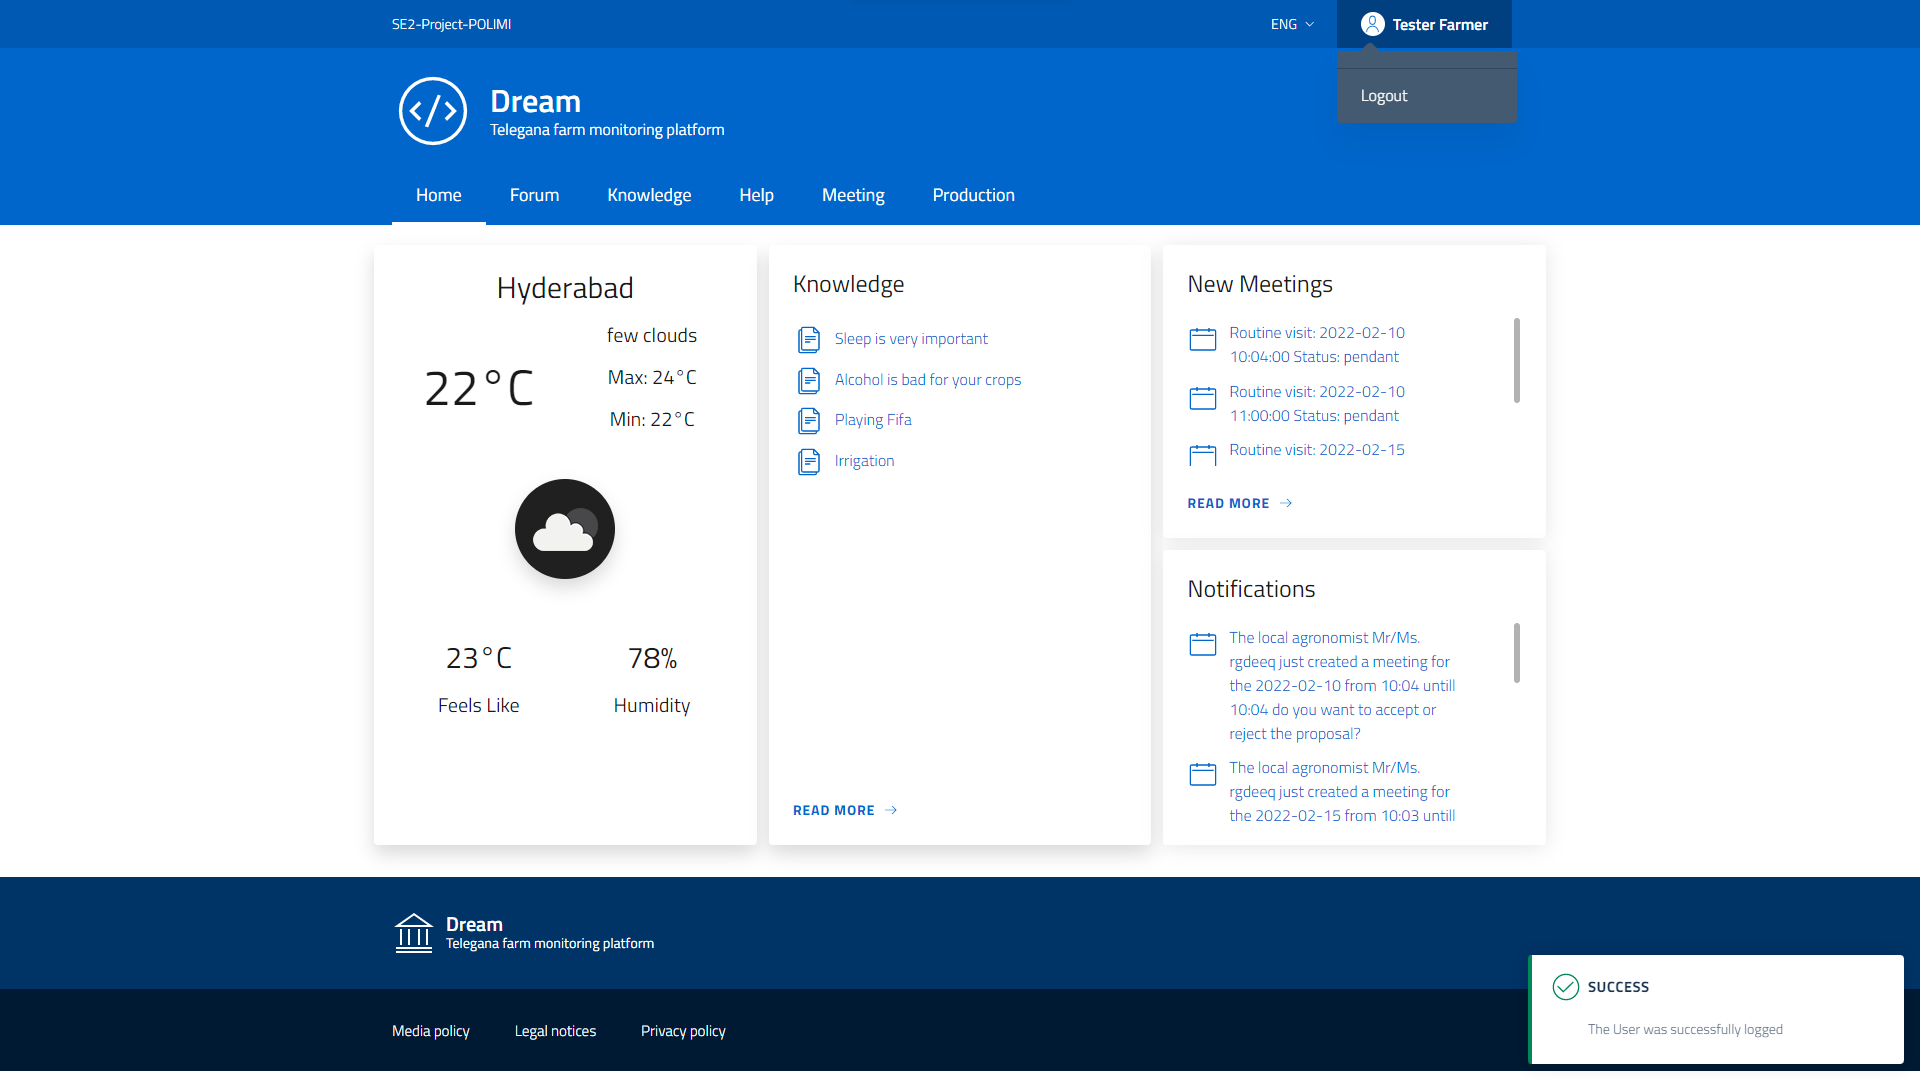
\includegraphics[width=\textwidth]{figures/farmers_home_page_log_out_dropdown.png}
        \caption{Unnecessary \textit{Logout} dropdown shown after a successful log in operation.}
        \label{fig:logout_dropdown}
    \end{figure}

    \item Some buttons display in inconvenient areas of the screen, which make them difficult to notice. An example of this issue is shown in the figure \ref{fig:button_placement}. Such unresponsiveness is also visible in the placement of the pop-up notifications when the page is zoomed out (example in the figure \ref{fig:unresponsive_design}).
    
    \begin{figure}[H]
        \centering
        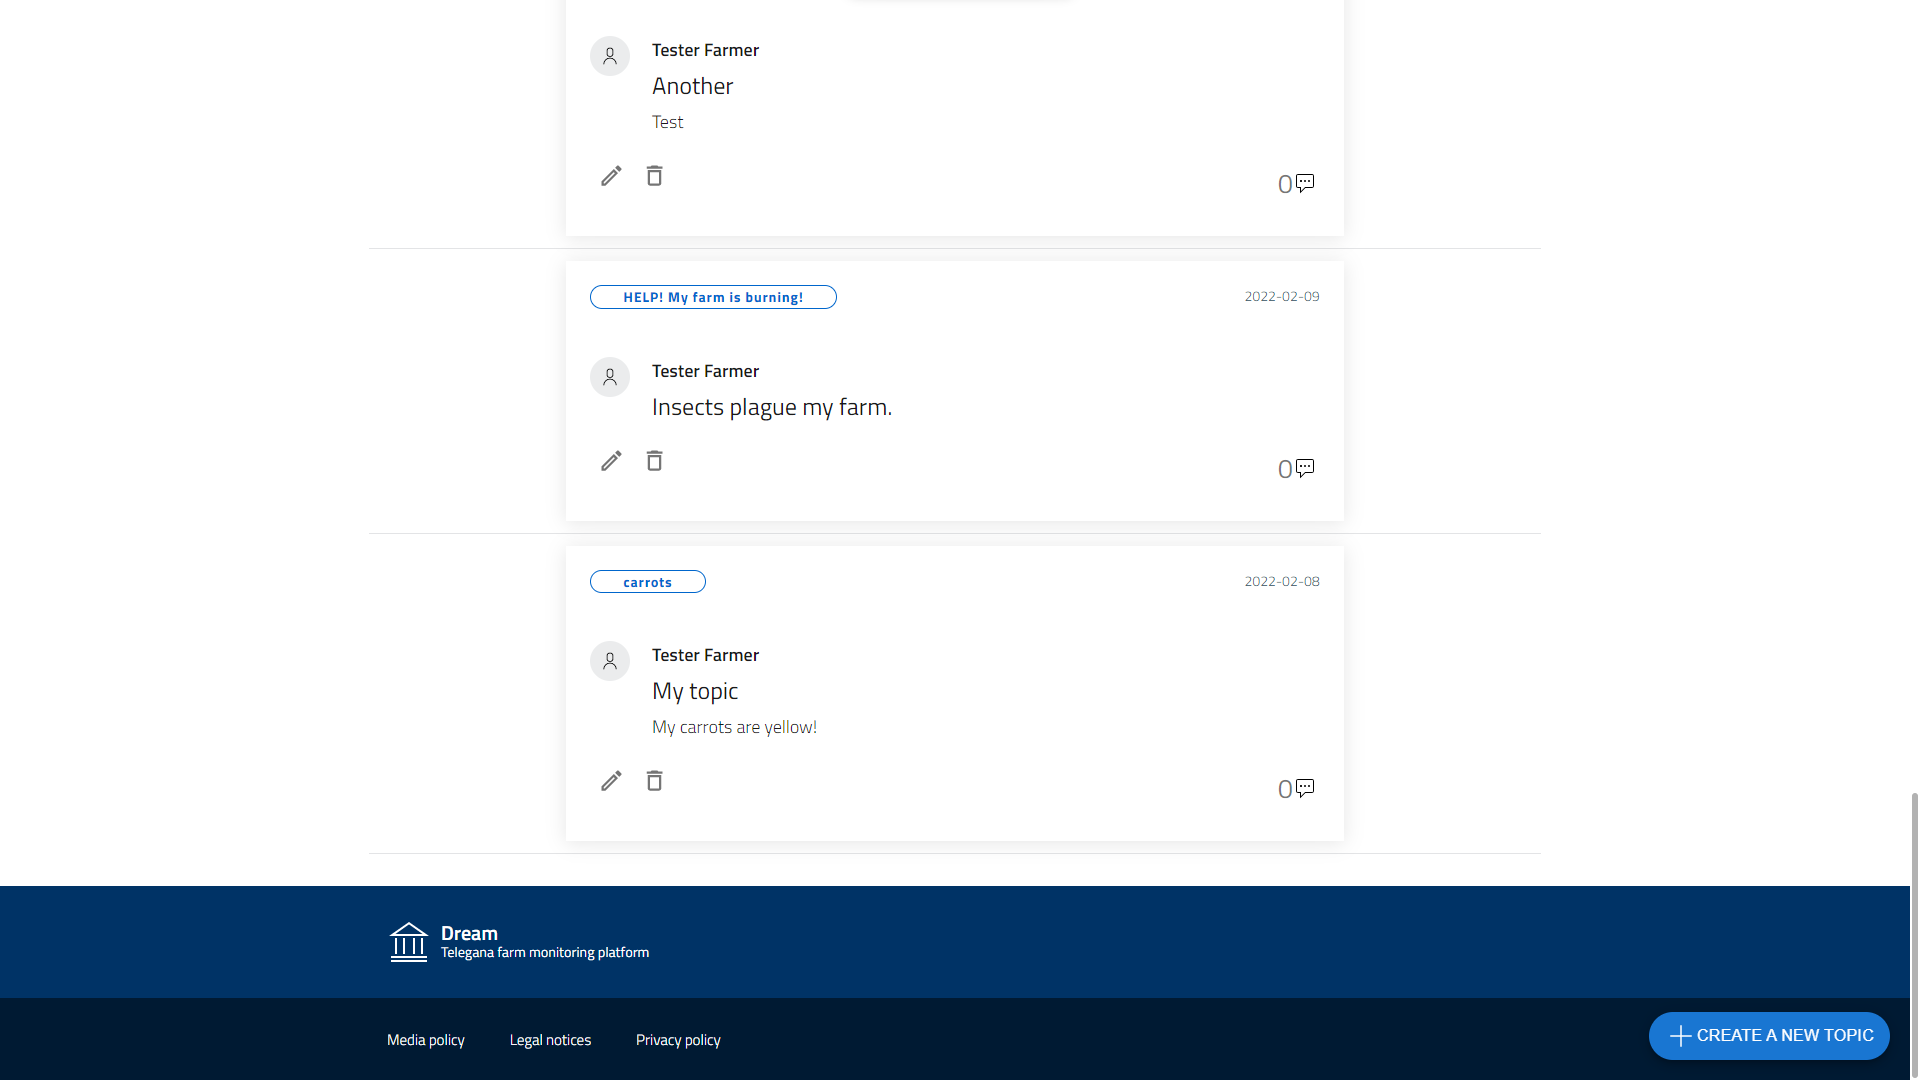
\includegraphics[width=\textwidth]{figures/button_placement.png}
        \caption{Inconvenient button placement example.}
        \label{fig:button_placement}
    \end{figure}

    \begin{figure}[H]
        \centering
        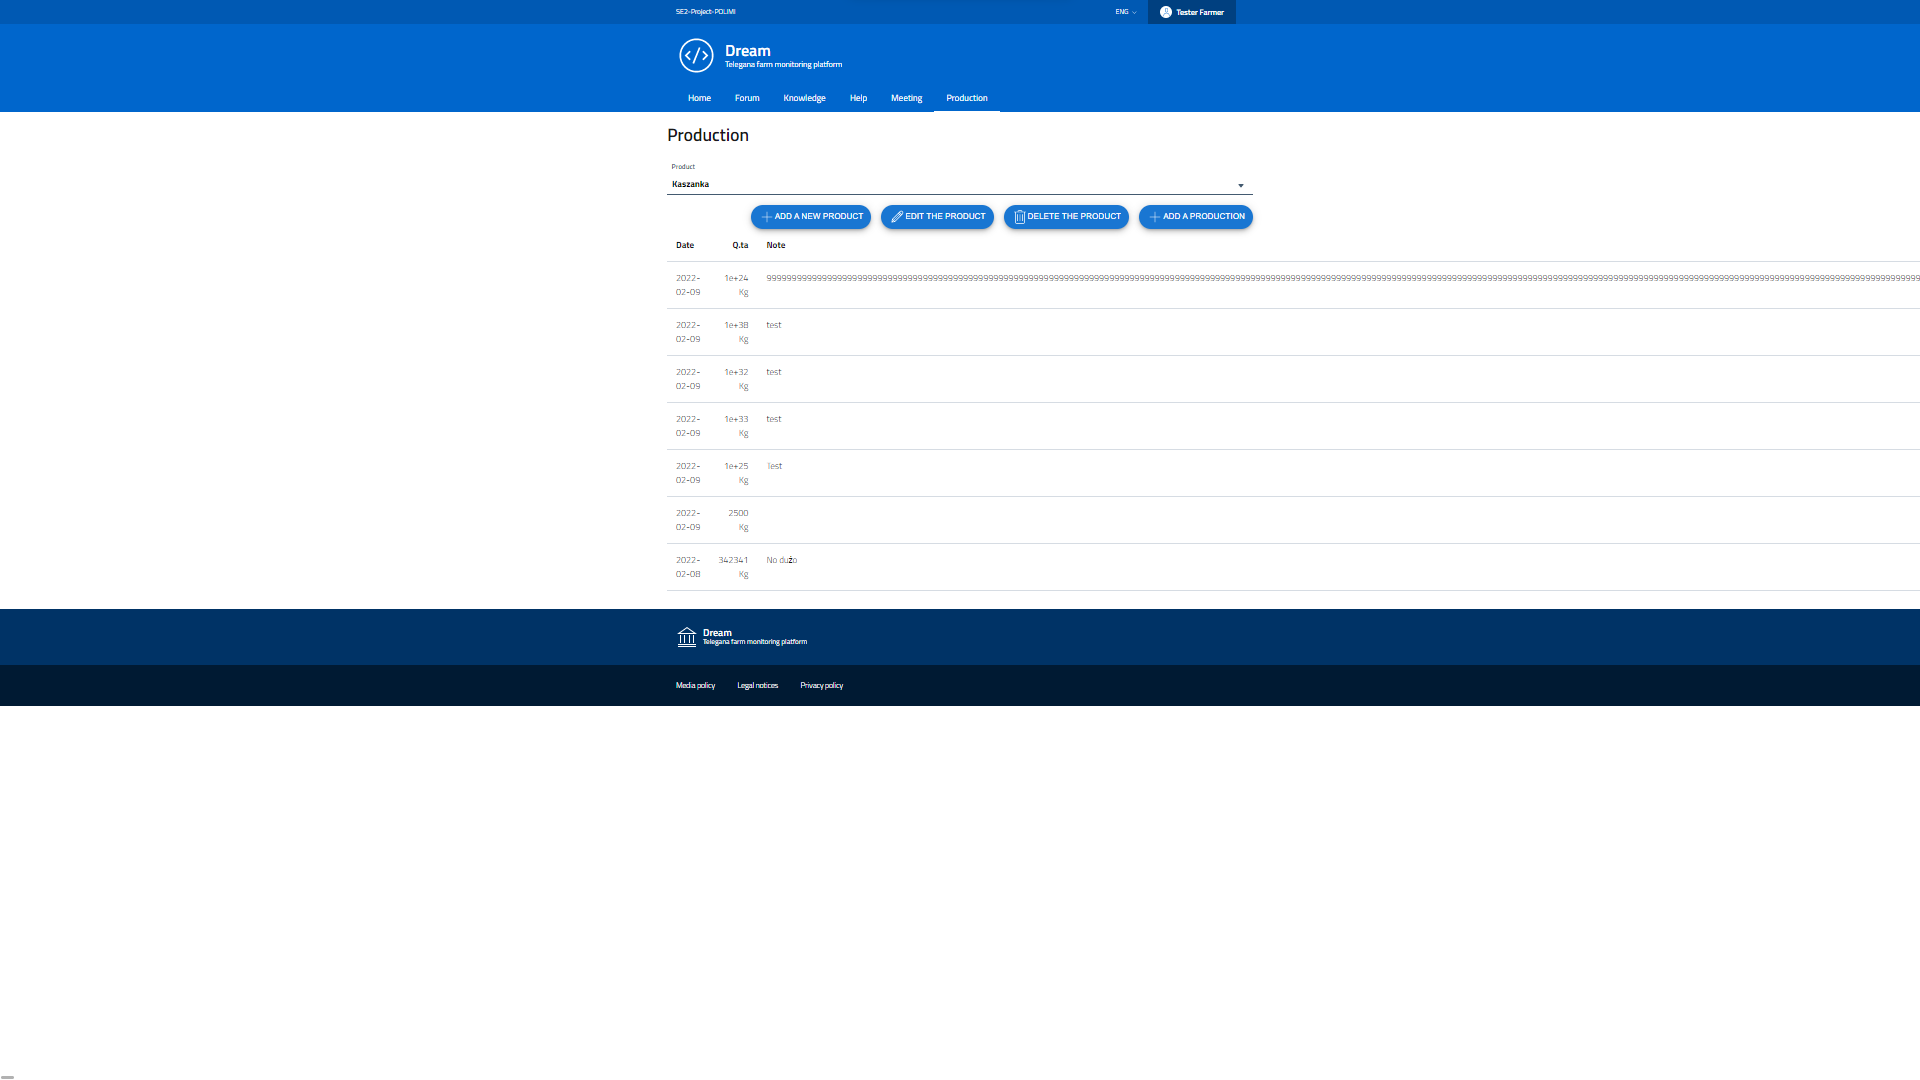
\includegraphics[width=\textwidth]{figures/very_long_input.png}
        \caption{Very long input breaks the page.}
        \label{fig:long_input}
    \end{figure}
    
    \item Some components do not scale well when given a long input string of characters. The text, instead of being wrapped, causes the page to become wider. This issue is depicted in the figure \ref{fig:long_input}.
    
    \begin{figure}[H]
        \centering
        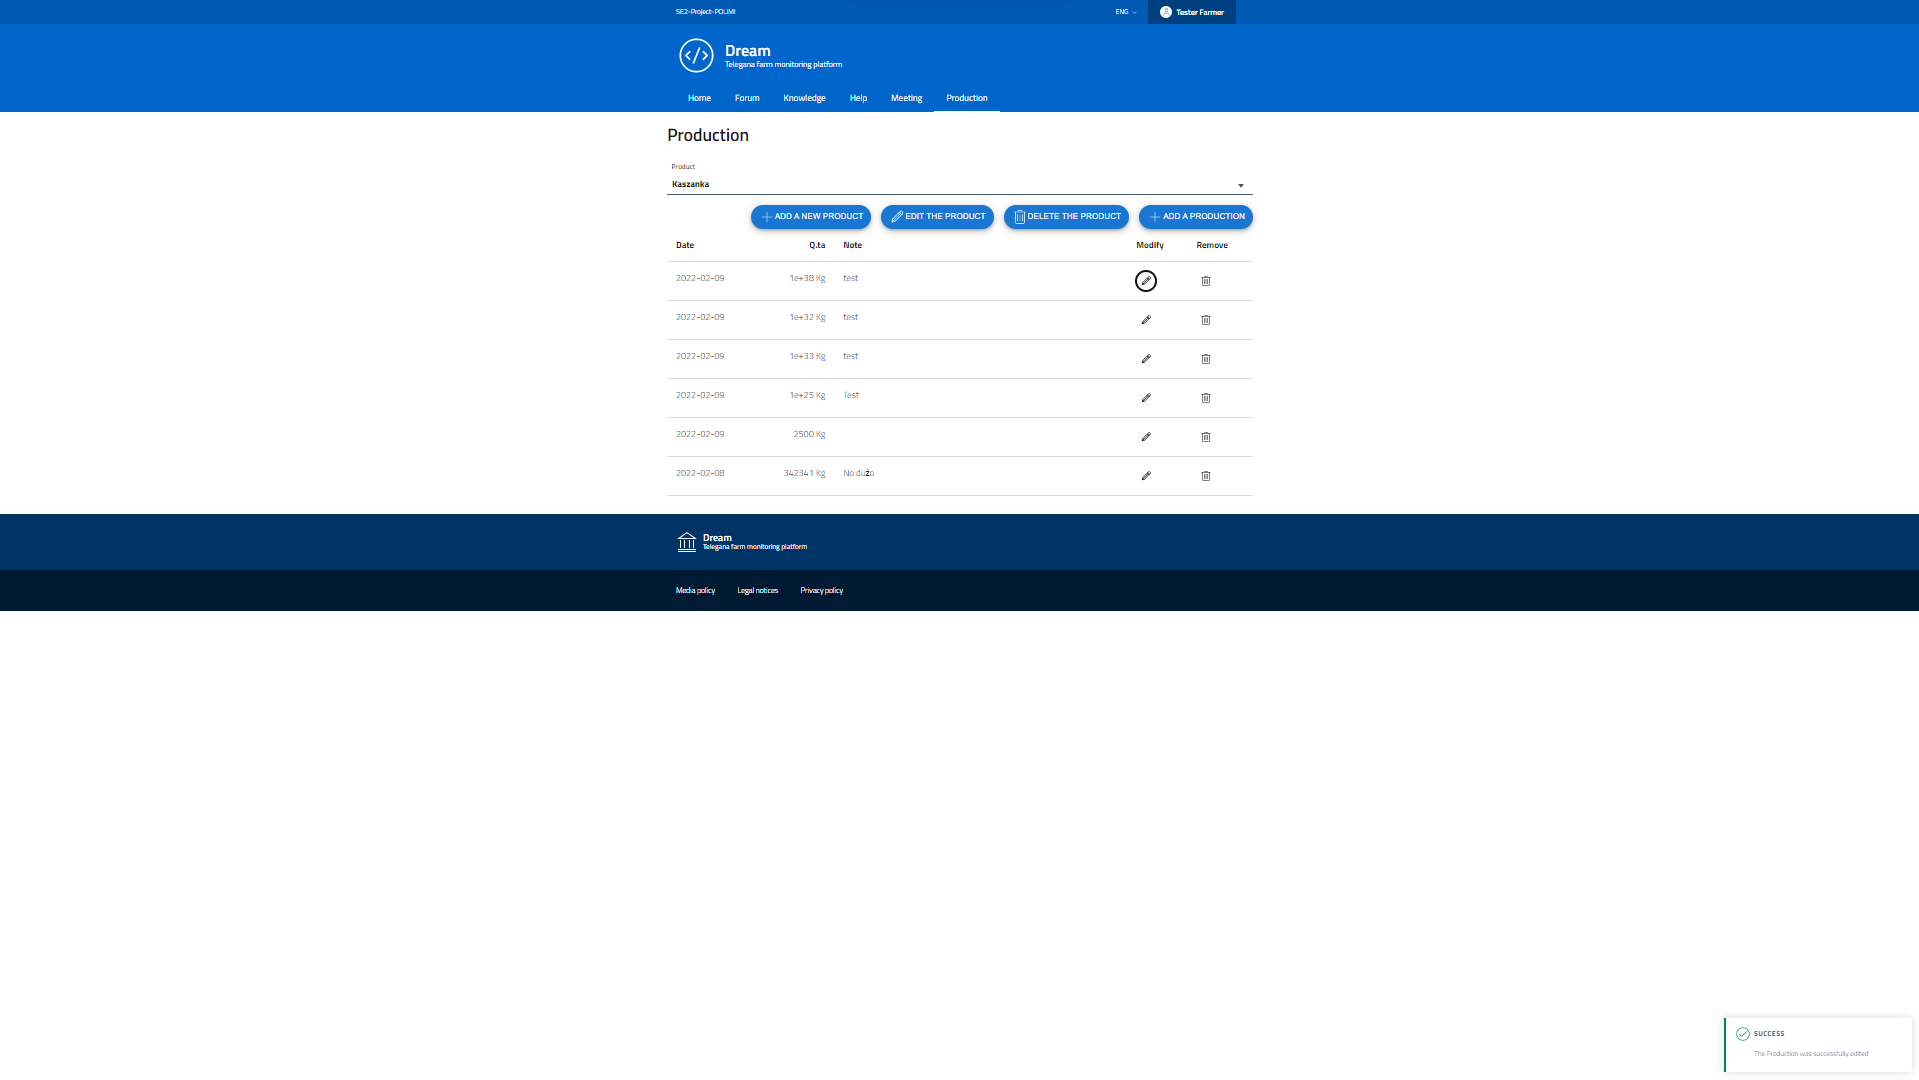
\includegraphics[width=\textwidth]{figures/unresponsive_design.png}
        \caption{An example of the design being unresponsive.}
        \label{fig:unresponsive_design}
    \end{figure}
\end{itemize}
